%%%%%%%%%%%%%%%%%%%%%%%%%%%%%%%%%%%%%%%%%
% Short Sectioned Assignment
% LaTeX Template
% Version 1.0 (5/5/12)
%
% This template has been downloaded from:
% http://www.LaTeXTemplates.com
%
% Original author:
% Frits Wenneker (http://www.howtotex.com)
%
% License:
% CC BY-NC-SA 3.0 (http://creativecommons.org/licenses/by-nc-sa/3.0/)
%
%%%%%%%%%%%%%%%%%%%%%%%%%%%%%%%%%%%%%%%%%

%----------------------------------------------------------------------------------------
%	PACKAGES AND OTHER DOCUMENT CONFIGURATIONS
%----------------------------------------------------------------------------------------

\documentclass[paper=a4, fontsize=11pt]{scrartcl} % A4 paper and 11pt font size

\usepackage[T1]{fontenc} % Use 8-bit encoding that has 256 glyphs
%\usepackage{fourier} % Use the Adobe Utopia font for the document - comment this line to return to the LaTeX default
\usepackage[english]{babel} % English language/hyphenation
\usepackage{amsmath,amsfonts,amsthm} % Math packages
\usepackage{mathtools} %More math! (For dscases)
\usepackage{hyperref} %HTML package
\usepackage{pgfplots} %Makes plots in LaTeX
\usepackage{tikz} %Also tikz?
\usepackage{bm} %makes vectors bold
\usepackage{bbm} %Blackboard bold 1
\usepgfplotslibrary{fillbetween}%Let's me fill between named plots
\usepackage{graphicx} %import pics

\usepackage[noend]{algpseudocode} %Algorithms
\usepackage{algorithm}

\graphicspath{ {Python\_figs/} }
\DeclareGraphicsExtensions{.pdf,.png,.jpg}
\usepackage{sectsty} % Allows customizing section commands
\allsectionsfont{ \normalfont\scshape} % Make all sections the default font and small caps


\renewcommand{\thesubsection}{\alph{subsection}} %Make subsections start with letters

\usepackage{fancyhdr} % Custom headers and footers
\pagestyle{fancyplain} % Makes all pages in the document conform to the custom headers and footers
\fancyhead{} % No page header - if you want one, create it in the same way as the footers below
\fancyfoot[L]{} % Empty left footer
\fancyfoot[C]{} % Empty center footer
\fancyfoot[R]{\thepage} % Page numbering for right footer
\renewcommand{\headrulewidth}{0pt} % Remove header underlines
\renewcommand{\footrulewidth}{0pt} % Remove footer underlines
\setlength{\headheight}{13.6pt} % Customize the height of the header

\numberwithin{equation}{section} % Number equations within sections (i.e. 1.1, 1.2, 2.1, 2.2 instead of 1, 2, 3, 4)
\numberwithin{figure}{section} % Number figures within sections (i.e. 1.1, 1.2, 2.1, 2.2 instead of 1, 2, 3, 4)
\numberwithin{table}{section} % Number tables within sections (i.e. 1.1, 1.2, 2.1, 2.2 instead of 1, 2, 3, 4)

\setlength\parindent{0pt} % Removes all indentation from paragraphs - comment this line for an assignment with lots of text
\usepackage{listings}
\lstset{language=Python}


\usepackage{tikz}
\usetikzlibrary{decorations.pathmorphing}
\usetikzlibrary{arrows}


%----------------------------------------------------------------------------------------
%	TITLE SECTION
%----------------------------------------------------------------------------------------

\newcommand{\horrule}[1]{\rule{\linewidth}{#1}} % Create horizontal rule command with 1 argument of height

\title{	Assignment 7}

\author{Benjamin Jakubowski} % Your name

\date{\normalsize\today} % Today's date or a custom date

\begin{document}

\maketitle % Print the title

%----------------------------------------------------------------------------------------
%	PROBLEM 1
%----------------------------------------------------------------------------------------
\section{BFS on figure 22.3 starting from $u$}

Using $u$ as a source in the graph shown in CLRS Figure 22.3 yields the following values for $d$ and $u$.

\begin{center}
\begin{tabular}{| c | c | c |}
\hline
	Vertex & $d$ & $\pi$ \\
\hline
	$u$ & 0 & \texttt{Nil} \\
\hline
	$t$ & 1 & $u$ \\
\hline
	$x$ & 1 & $u$ \\
\hline
	$y$ & 1 & $u$ \\
\hline
	$w$ & 2 & $t^1$ \\
\hline
	$s$ & 3 & $w$\\
\hline
	$r$ & 4 & $s$ \\
\hline
	$v$ & 5 & $r$ \\
\hline
\end{tabular} \\
\end{center}
$^1$Note this assumes the adjacency list for $G.E[u]$ is $[t, x, y]$, such that $t$ is the first vertex enqueued from $u$ and as such is the parent for $w$.

%----------------------------------------------------------------------------------------
%	PROBLEM 2
%----------------------------------------------------------------------------------------

\section{Efficient algorithm to compute the diameter of a tree}

An algorithm to compute the diameter of a tree is:

\begin{algorithmic}
\Function{diameter}{T}
	\State Pick a vertex $s$ from T.V
	\State Let $u$ be the last vertex discovered in BFS(T, s)
	\State Let $v$ be the last vertex discovered in BFS(T, u)
	\State \Return d(u, v) (i.e. v.d following second BFS)
\EndFunction
\end{algorithmic}

We now prove the correctness of this algorithm.

Let $x$ and $y$ be vertices in $T.V$ such that $d(x,y) = diam(T)$, and let $s$ be the arbitrary vertex selected from $T.V$ to initialize the first BST.

Then let $u$ be the last vertex discovered in BFS(T, $s$), such that (following the first BFS)
\[u.d = \max_{w \in T.V} w.d\]
The let $v$ be the last vertex discovered in BFS(T, $u$), such that (following the second BFS)
\[v.d = \max_{w \in T.V} w.d\]

Our claim is that $v.d = d(u, v) = diam(T)$. Before we begin, note since $T$ is a tree, there is a single simple path connecting any two vertices in $T$. Thus, going forward, mention of paths and distances between two vertices assume this uniqueness. Additionally, note if we pick $s$ to be either $x$ or $y$, then our algorithm clearly return $d(x,y)$ and is correct. Hence, assume we pick some $s \ne x, y$. \\
 
Now consider the path between $x$ and $y$, and it's relationship to $s$. Note the paths from $s$ to $x$ and from $s$ to $y$ must both include some $a$ in $x \sim y$, $a \ne x, y$.

\begin{center}
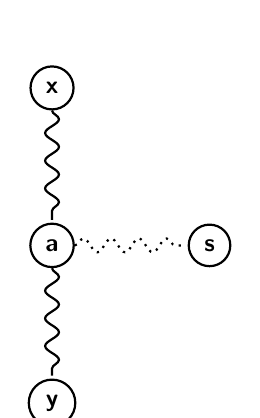
\begin{tikzpicture}[>=stealth',shorten >=1pt,auto,node distance=2cm, thick,main node/.style={circle,draw,font=\sffamily\small\bfseries}]

  \node[main node] (x) {x};
  \node[main node] (a) [below of=x] {a};
  \node[main node] (s) [right of=a] {s};
  \node[main node] (y) [below of=a] {y};
  
  \path[every node/.style={font=\sffamily\tiny}]
    (x) edge [decorate, decoration=snake] node [left] {} (a)
    (a) edge [dotted, decorate, decoration=snake] node [above right] {} (s)
         edge [decorate, decoration=snake] node [left] {} (y);
    
\end{tikzpicture}
\end{center}

Otherwise, $diam(T) \ne d(x,y)$, since we can construct a longer path (either the path $s \sim x = a \sim y$ or $s \sim y = a \sim x$, and again these are then unique simple paths $s \sim y$ or $s \sim x$ since $T$ is a tree).

\begin{center}
\begin{tabular}{ c c }

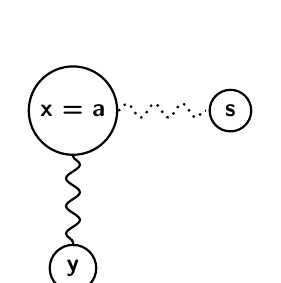
\begin{tikzpicture}[>=stealth',shorten >=1pt,auto,node distance=2cm, thick,main node/.style={circle,draw,font=\sffamily\small\bfseries}]

  \node[main node] (x) {x = a};
  \node[main node] (s) [right of=x] {s};
  \node[main node] (y) [below of=x] {y};
  
  \path[every node/.style={font=\sffamily\tiny}]
    (x) edge [decorate, decoration=snake] node [left] {} (y)
         edge [dotted, decorate, decoration=snake] node [above right] {} (s);
    
\end{tikzpicture}
&
\begin{tikzpicture}[>=stealth',shorten >=1pt,auto,node distance=2cm, thick,main node/.style={circle,draw,font=\sffamily\small\bfseries}]

  \node[main node] (x) {x};
  \node[main node] (s) [right of=y] {s};
  \node[main node] (y) [below of=x] {y = a};
  
  \path[every node/.style={font=\sffamily\tiny}]
    (y) edge [decorate, decoration=snake] node [left] {} (x)
         edge [dotted, decorate, decoration=snake] node [above right] {} (s);
    
\end{tikzpicture}
\\
\end{tabular}
\end{center}

Additionally, note while we assume $s \ne x,y$, it is possible $s = a$. \\

Next, consider the path between $u$ and $v$, and it's relationship to $s$. Note if $s \ne u, v$ the paths $s \sim u$ and $s \sim v$ must both include some $b$ in the interior of $u \sim v$.

\begin{center}
\begin{tikzpicture}[>=stealth',shorten >=1pt,auto,node distance=2cm, thick,main node/.style={circle,draw,font=\sffamily\small\bfseries}]

  \node[main node] (y) {u};
  \node[main node] (a) [below of=x] {b};
  \node[main node] (s) [right of=a] {s};
  \node[main node] (y) [below of=a] {v};
  
  \path[every node/.style={font=\sffamily\tiny}]
    (x) edge [decorate, decoration=snake] node [left] {} (a)
    (a) edge [dotted, decorate, decoration=snake] node [above right] {} (s)
         edge [decorate, decoration=snake] node [left] {} (y);
    
\end{tikzpicture}
\end{center}

If it did not, we would have one of two contradictions:
\begin{itemize}
\item $d(s,u) \ne \max_{w \in T.V} d(s, w)$, since we can construct a longer path $s \sim u = b \sim v$. This contradictory path is illustrated below

\begin{center}
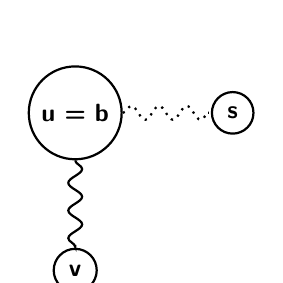
\begin{tikzpicture}[>=stealth',shorten >=1pt,auto,node distance=2cm, thick,main node/.style={circle,draw,font=\sffamily\small\bfseries}]

  \node[main node] (u) {u = b};
  \node[main node] (s) [right of=u] {s};
  \node[main node] (v) [below of=u] {v};
  
  \path[every node/.style={font=\sffamily\tiny}]
    (u) edge [decorate, decoration=snake] node [left] {} (v)
         edge [dotted, decorate, decoration=snake] node [above right] {} (s);
    
\end{tikzpicture}
\end{center}

\item $d(u,v) \ne \max_{w \in T.V} d(u, w)$, since we can construct a longer path $u \sim v = b \sim s$. This contradictory path is also shown below.

\begin{center}
\begin{tikzpicture}[>=stealth',shorten >=1pt,auto,node distance=2cm, thick,main node/.style={circle,draw,font=\sffamily\small\bfseries}]

  \node[main node] (u) {u};
  \node[main node] (s) [right of=v] {s};
  \node[main node] (v) [below of=u] {v = b};
  
  \path[every node/.style={font=\sffamily\tiny}]
    (v) edge [decorate, decoration=snake] node [left] {} (u)
         edge [dotted, decorate, decoration=snake] node [above right] {} (s);
    
\end{tikzpicture}
\end{center}
\end{itemize}

Now we proceed to show this yields $diam(t)  = d(u,v)$.

First note
\[d(s, b) + d(b, u) \geq d(s,a) + d(a,x)\]
otherwise the first BFS does not find $u$.
Additionally, 
\[d(b, v) \geq d(b,a) + d(a,y)\]
otherwise the second BFS does not find $v$.

But then combining these inequalities yields
\begin{align*}
d(s,b) + \underbrace{d(b,u) + d(b,v)}_{=d(u,v)} &\geq d(s,a) + d(b,a) + \underbrace{d(a,x) + d(a,y)}_{d(x,y)} \\
\implies \qquad{} d(s,b) + d(u,v) &\geq d(x,y) + d(s,a) + d(b,a)
\end{align*}

But note $d(s,b) \leq d(s,a) + d(b,a)$ since $s \sim a \sim b$ is a (potentially non-simple) path $s \sim b$.

This, we conclude
\begin{align*}
d(s,b) + d(u,v) &\geq d(x,y) + d(s,a) + d(b,a) \\
\implies \qquad{}  d(u, v) &\geq d(x,y)
\end{align*}

But by assumption $d(x,y) = diam(T)$, so $d(x,y) = \max_{s,t \in T.V} d(s,t)$. Hence, $d(x,y) = d(u,v) = diam(T)$.

Next we consider the running time of the algorithm. Since it is involves running BFS twice, it is just $O(BFS) = O(V + E)$.

%----------------------------------------------------------------------------------------
%	PROBLEM 3
%----------------------------------------------------------------------------------------

\section{DFS on graph of Figure 22.6}
DFS on the graph of Figure 22.6 produces the discovery and finishing times and edge classifications 

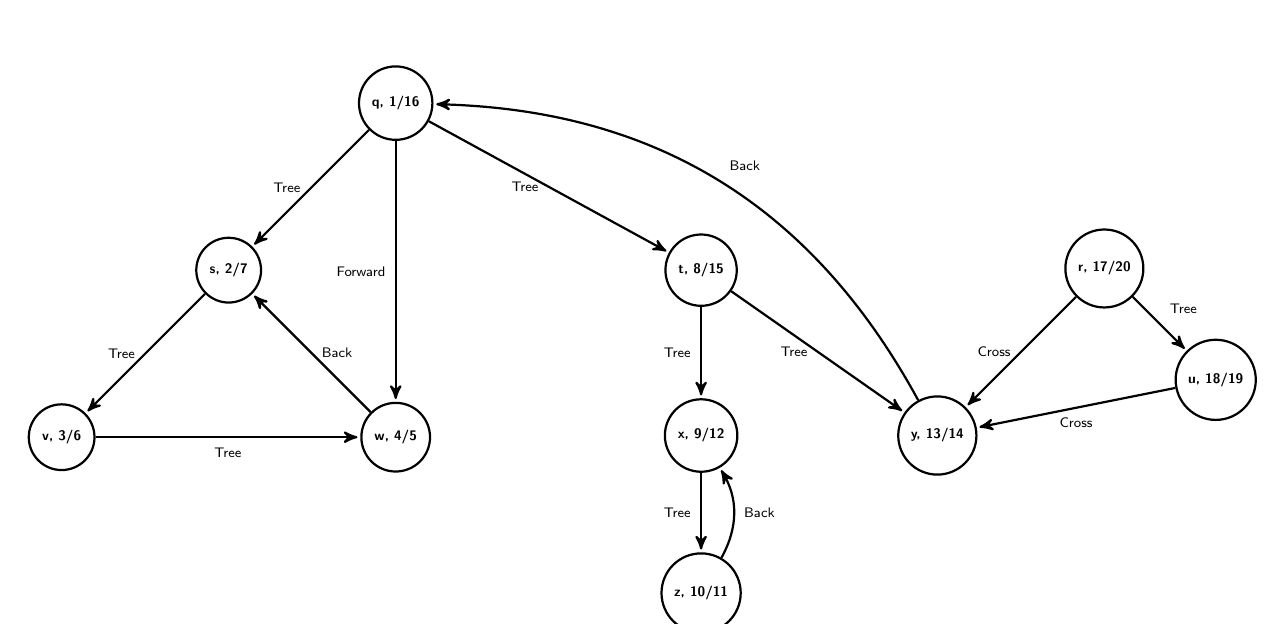
\begin{tikzpicture}[->,>=stealth',shorten >=1pt,auto,node distance=3cm,
                    thick,main node/.style={circle,draw,font=\sffamily\tiny\bfseries}]

  \node[main node] (q) {q, 1/16};
  \node[main node] (s) [below left of=q] {s, 2/7};
  \node[main node] (t) [right of=s,node distance=6cm] {t, 8/15};
  \node[main node] (x) [below of=t, node distance=2.1cm] {x, 9/12};
  \node[main node] (y) [right of=x,node distance=3cm] {y, 13/14};
  \node[main node] (r) [above right of=y]{r, 17/20};
  \node[main node] (u) [below right of=r, node distance=2cm] {u, 18/19};
  \node[main node] (v) [below left of=s] {v, 3/6};
  \node[main node] (w) [below right of=s] {w, 4/5};
  \node[main node] (z) [below of=x, node distance=2cm] {z, 10/11};

  \path[every node/.style={font=\sffamily\tiny}]
    (q) edge node [left] {Tree} (s)
        edge node [left] {Tree} (t)
        edge node [left] {Forward} (w)
    (r) edge node [above right] {Tree} (u)
        edge node [left] {Cross} (y)
    (s) edge node [left] {Tree} (v)
    (v) edge node [below] {Tree} (w)
    (w) edge node [right] {Back} (s)
    (t) edge node [left] {Tree} (x)
    	edge node [left] {Tree} (y)
    (x) edge node [left] {Tree} (z)
    (z) edge [bend right] node [right] {Back} (x)
    (u) edge node [below] {Cross} (y)
    (y) edge [bend right] node [above right] {Back} (q);
    
\end{tikzpicture}

%----------------------------------------------------------------------------------------
%	PROBLEM 4
%----------------------------------------------------------------------------------------

\section{Ordering of vertices produced by \texttt{Topological-Sort}}

When \texttt{Topological-Sort} isrun on the DAG of Figure 22.8, under the assumption of Exercise 22.3-2, the following ordering is obtained:
\begin{enumerate}
\item p
\item n
\item o
\item s
\item m
\item r
\item y
\item v
\item x
\item w
\item z
\item u
\item z
\item t
\end{enumerate}


%----------------------------------------------------------------------------------------
%	PROBLEM 5
%----------------------------------------------------------------------------------------
\section{Determining whether or not there's a cycle}

Consider an undirected graph $G = (V, E)$. We give an $O(V)$ algorithm that determines whether or not the graph contains a cycle. We first make and prove a couple of claims:\\

\textbf{Claim 1}: Any acyclic graph has $|E| \leq |V| - 1$ edges.\\

First, note that the graph $G$ clearly has a cycle if $|E| \geq |V|$. To see this, note that if a connected graph has $|E| = |V| - 1$, then $G$ is acyclic. Therefore, a disconnected acyclic graph has $|E| < |V| - 1$, since it can be constructed by removing connecting edges from a connected acyclic graph. Thus, any acyclic graph has $|E| \leq |V| - 1$ edges.\\

\textbf{Claim 2}: If $|E| < |V|$, \texttt{DFS}$(G) = O(|V|)$\\

Recall DFS is $O(V + E)$. However, if $|E| < |V|$, then substitution yields
\[O(V + E) = O(V + V) = O(V)\]

With these two claims in mind, we present an $O(V)$ algorithm for detecting cycles in an undirected graph $G$. The algorithm essentially:
\begin{enumerate}
\item Checks if $|E| \geq |V|$. If so, then $G$ has cycles
\item If not, it runs a modified DFS (which runs in $O(|V|)$- see claim 2), returning true if a cycle is found (i.e. there is a back edge from $u$ to $v$).

The algorithm is presented below:

\end{enumerate}

\begin{algorithmic}
\Function{has\_cycles}{G}
	\State V = 0 \Comment{Counter for number of vertices}
	\State E = 0 \Comment{Counter for number of edges}
	\For {v in G.V}
		\State V++
	\EndFor
	\For {v in G.V}
		\For {e in G.E[v]}
			\State E++
			\If {E $\geq$ V}
				\State \Return true
			\EndIf
		\EndFor
	\EndFor
	\State \Return modified\_DFS(G) \Comment{Only reached if $E < V$}
\EndFunction
\end{algorithmic}

\begin{algorithmic}
\Function{modified\_DFS}{G}
	\For {u in G.V}
		\State u.color == White
		\State u.$\pi$ = Nil
	\EndFor
	\State time = 0
	\For {u in G.V}
		\If {u.color == white}
			\If{modified\_DFS\_visit(G,u)}
				\State \Return true
			\EndIf
		\EndIf
	\EndFor
	\State \Return false \Comment{Only reached if no cycles}
\EndFunction
\end{algorithmic}

\begin{algorithmic}
\Function{modified\_DFS\_visit}{G, u}
	\State time = time + 1
	\State u.d = time
	\State u.color = Gray
	\For {v in G.E[u]}
		\If {v.color == White}
			\State v.$\pi$ = u
			\If{modified\_DFS\_visit(G, v)}
				\State \Return true
			\EndIf
		\Else \Comment {v.color != White}
			\If {(v != u.$\pi$) or (v.$\pi$ != u)} \Comment{(u,v) must complete a cycle}
				\State \Return True
			\EndIf
		\EndIf
	\EndFor
	\State u.color = black
	\State time = time + 1
	\State u.f = time
	\State \Return false
\EndFunction
\end{algorithmic}

%----------------------------------------------------------------------------------------
%	PROBLEM 7
%----------------------------------------------------------------------------------------
\section{\texttt{Strongly-Connected-Components} on graph of Figure 22.6}

First, the finishing times are given in the graph shown for problem three. The nodes finish (in decreasing order):

\begin{enumerate}
\item r
\item u
\item q
\item t
\item y
\item x
\item z
\item s
\item v
\item w
\end{enumerate}

When DFS is run a second time, visiting the vertices in this order, we obtain the following forest of strongly connected components:\

\begin{center}
\begin{tikzpicture}[>=stealth',shorten >=1pt,auto,node distance=2cm,
                    thick,main node/.style={circle,draw,font=\sffamily\small\bfseries}]

 \node[main node] (r) {r};
  \node[main node] (u) [right of=r] {u};
  \node[main node] (q) [right of=u] {q};
  \node[main node] (t) [right of=q] {t};
  \node[main node] (y) [right of=t] {y};
  \node[main node] (x) [right of=y]{x};
  \node[main node] (z) [below of=x] {z};
  \node[main node] (s) [right of=x] {s};
  \node[main node] (w) [below of=s] {w};
  \node[main node] (v) [below of=w] {v};

  \path[every node/.style={font=\sffamily\tiny}]
    (x) edge node {} (z)
    (s) edge node {} (w)
    (w) edge node {} (v)
    ;
  
\end{tikzpicture}
\end{center}

%----------------------------------------------------------------------------------------
%	PROBLEM 7
%----------------------------------------------------------------------------------------
\section{BFS tree edge classification}

\subsection{BFS of undirected graph}

First, throughout we assume without loss of generality $u$ is discovered before $v$. If not, swap the labels "$u$" and "$v$" and the proof holds.

\subsubsection{No back edges and no forward edges}

Consider a BFS tree of an undirected graph. Consider two vertices $u$ and $v$ connected by edge $(u,v)$. This cannot be a forward edge, since if $v$ is a descendant of $u$ and there exists an edge $(u,v)$, $v \in G.Adj[u]$ and so $v$ is discovered in the inner loop on lines 12-17 in the BFS algorithm given on page 595 of CLRS. Thus, $(u,v)$ must be a tree edge and not a forward edge. Finally, since we are considering an undirected graph, back edges and forward edges are the same; thus we immediately have that there are also no back edges.

\subsubsection{A tree edge $(u,v)$ has $v.d = u.d + 1$}

Since $v$ is in $G.Adj[u]$, $v$ is discovered in the inner loop on lines 12-17 in the BFS algorithm given on page 595 of CLRS. Thus, on line 15 we assign $v.d = u.d + 1$.

\subsubsection{A cross edge $(u,v)$ has $v.d = u.d$ or $u.d + 1$}

Cross edges are edges between vertices in in the BFS tree, where one vertex is not an ancestor of the other in the tree. First, note an edge $(u,v)$ is a cross edge if an only if it is not a tree edge (since we have previously shown there are no forward or back edges in an undirected graph's BFS tree).

Since $(u,v)$ is not a tree edge, $v$ must have been discovered (enqueued) from some vertex $x \ne u$. This vertex $x$ must have been enqueued and dequeued before $u$; otherwise, $v$ would have been discovered from $u$ and $(u,v)$ would be a tree edge.

But then at some point (recalling the assumption $u$ is discovered before $v$) the queue $Q$ must have contained
\[Q = [v_{start}, \cdots, x, \cdots, u, \cdots, v, \cdots, v_{end}]\]

Then, since $u$ and $v$ were in the queue $Q$ at the same time, by lemma 22.3
\[v_{start}.d + 1 \geq v_{end}.d \geq v.d \geq u.d \geq v_{start}\]

so
\[
v.d =
\begin{cases}
	u.d \\
	u.d + 1
\end{cases}
\]

\subsection{BFS of directed graph}
Again we assume without loss of generality $u$ is discovered before $v$.

\subsubsection{No forward edges}

Consider a BFS tree of a directed graph. Consider two vertices $u$ and $v$ connected by edge $(u,v)$. This cannot be a forward edge, since if $v$ is a descendant of $u$ and there exists an edge $(u,v)$, $v \in G.Adj[u]$ and so $v$ is discovered in the inner loop on lines 12-17 in the BFS algorithm given on page 595 of CLRS. Thus, $(u,v)$ must be a tree edge and not a forward edge. 

\subsubsection{A tree edge $(u,v)$ has $v.d = u.d + 1$}

Since $v$ is in $G.Adj[u]$, $v$ is discovered in the inner loop on lines 12-17 in the BFS algorithm given on page 595 of CLRS. Thus, on line 15 we assign $v.d = u.d + 1$.

\subsubsection{A cross edge $(u,v)$ has $v.d \leq u.d + 1$}

Again, cross edges are edges between vertices in in the BFS tree, where one vertex is not an ancestor of the other in the tree. Let $(u,v)$ be a cross edge. Then again since $(u,v)$ is not a tree edge, $v$ must have been discovered before $u$ was dequeued; otherwise, $v$ would have been discovered from $u$ and $(u,v)$ would be a tree edge.

But then $v.d \leq u.d + 1$, since at the time $u$ is dequeued $v$ is either
\begin{itemize}
\item \textbf{Case 1}: In the queue, but then by lemma 22.3 $u$ and $v$ were in the queue at the same time (with $v$ after $u$), so $v.d \leq u.d + 1$.
\item \textbf{Case 2}: Already out of the queue, but then clearly by the monotonicity of $d$ values in the queue $v.d \leq u.d$.
\end{itemize}

In either case, $v.d \leq u.d + 1$.

\subsubsection{A back edge $(u,v)$ has $0 \leq v.d \leq u.d$}

if $(u,v)$ is back edge, then $v$ must have been discovered before $u$; otherwise, when $u$ is dequeued $v$ would still be white, and then $v$ would be discovered from $u$, making $(u,v)$ a tree edge.

But then at the time $u$ is enqueued, by corollary 22.4, we clearly have $v.d \leq u.d$. Finally, note for all $w \in V, w.d \geq 0$. Thus, we have
\[0 \leq v.d \leq u.d\]

%----------------------------------------------------------------------------------------
\end{document}